\chapter{Literature Review} \label{chapter_three}

Previous chapter laid out the foundations for video stabilization and motion estimation. We also made the case for the techniques and algorithms chosen in this work. Now, this chapter includes some of the state-of-the-art methods for digital video stabilization and pose estimation. 

\section{Digital Video Stabilization}
Various sensor based digital image stabilization techniques have been developed over the years using both classical and data-driven approaches. These techniques are limited to rotational motion compensation or using image data.

\subsection{5D Video Stabilization through Sensor Vision Fusion}
This research aims to overcome the challenge of going beyond 3D stabilization (rotation only) by also including translational motion in their image stabilization algorithm for smartphones. The proposed 5D stabilization is achieved by carefully combining sensor based 3D rotation stabilization and vision based 2D translation stabilization \citep{zhuang20195d}. Figure \ref{fig:5d_stab} shows the block diagram for this approach. This method is promising as it deals with translational motion as well but does so using image features and hence cannot be used for our use case.

\begin{figure}
    \centering
    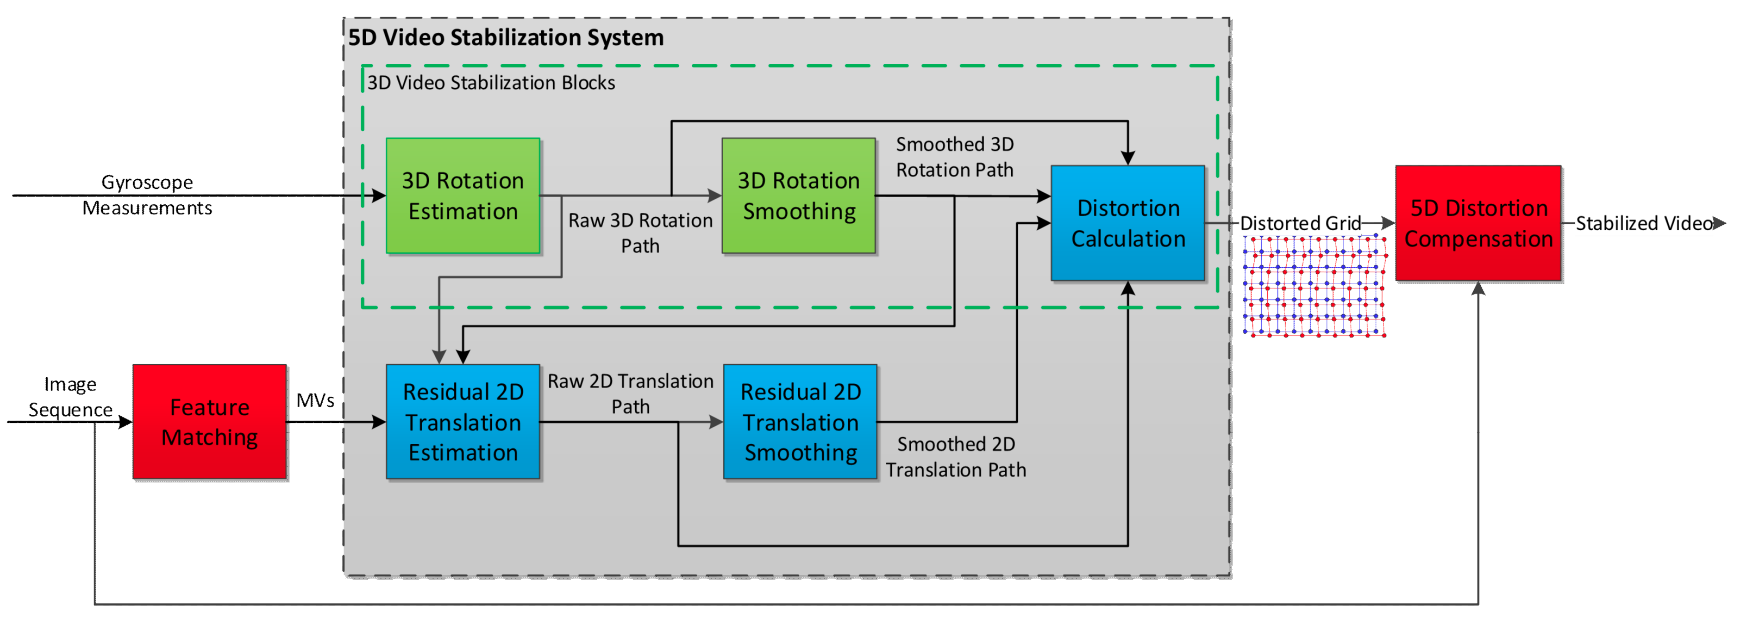
\includegraphics[scale=0.21]{images/fig_chapter3/5d_stab.png}
    \caption{Block diagram for proposed 5D video stabilization system \citep{zhuang20195d}} 
    \label{fig:5d_stab}
\end{figure}

\subsection{Deep Online Fused Video Stabilization}
This work aims at stabilizing videos using \textit{Gyroscope} data as well as \textit{Optical Flow} through unsupervised learned \citep{deep_opti_stab}. Instead of pose estimation, warping grid calculation and image warping the aim here is to directly warp the image based input data (images and gyroscope data) as shown in figure \ref{fig:deep_stab}. The results seem to outperform some of the previous state-of-the-art methods present before it. Although very promising this method cannot be used in our case as we want our algorithm to be image invariant based on reasons discussed in section \ref{sec:software_motion_estimation}. It also has a component of finding optical flow for each frame using a different neural network which makes this algorithm very computationally expensive and hence not usable all computers/hardware.

\begin{figure}[H]
    \centering
    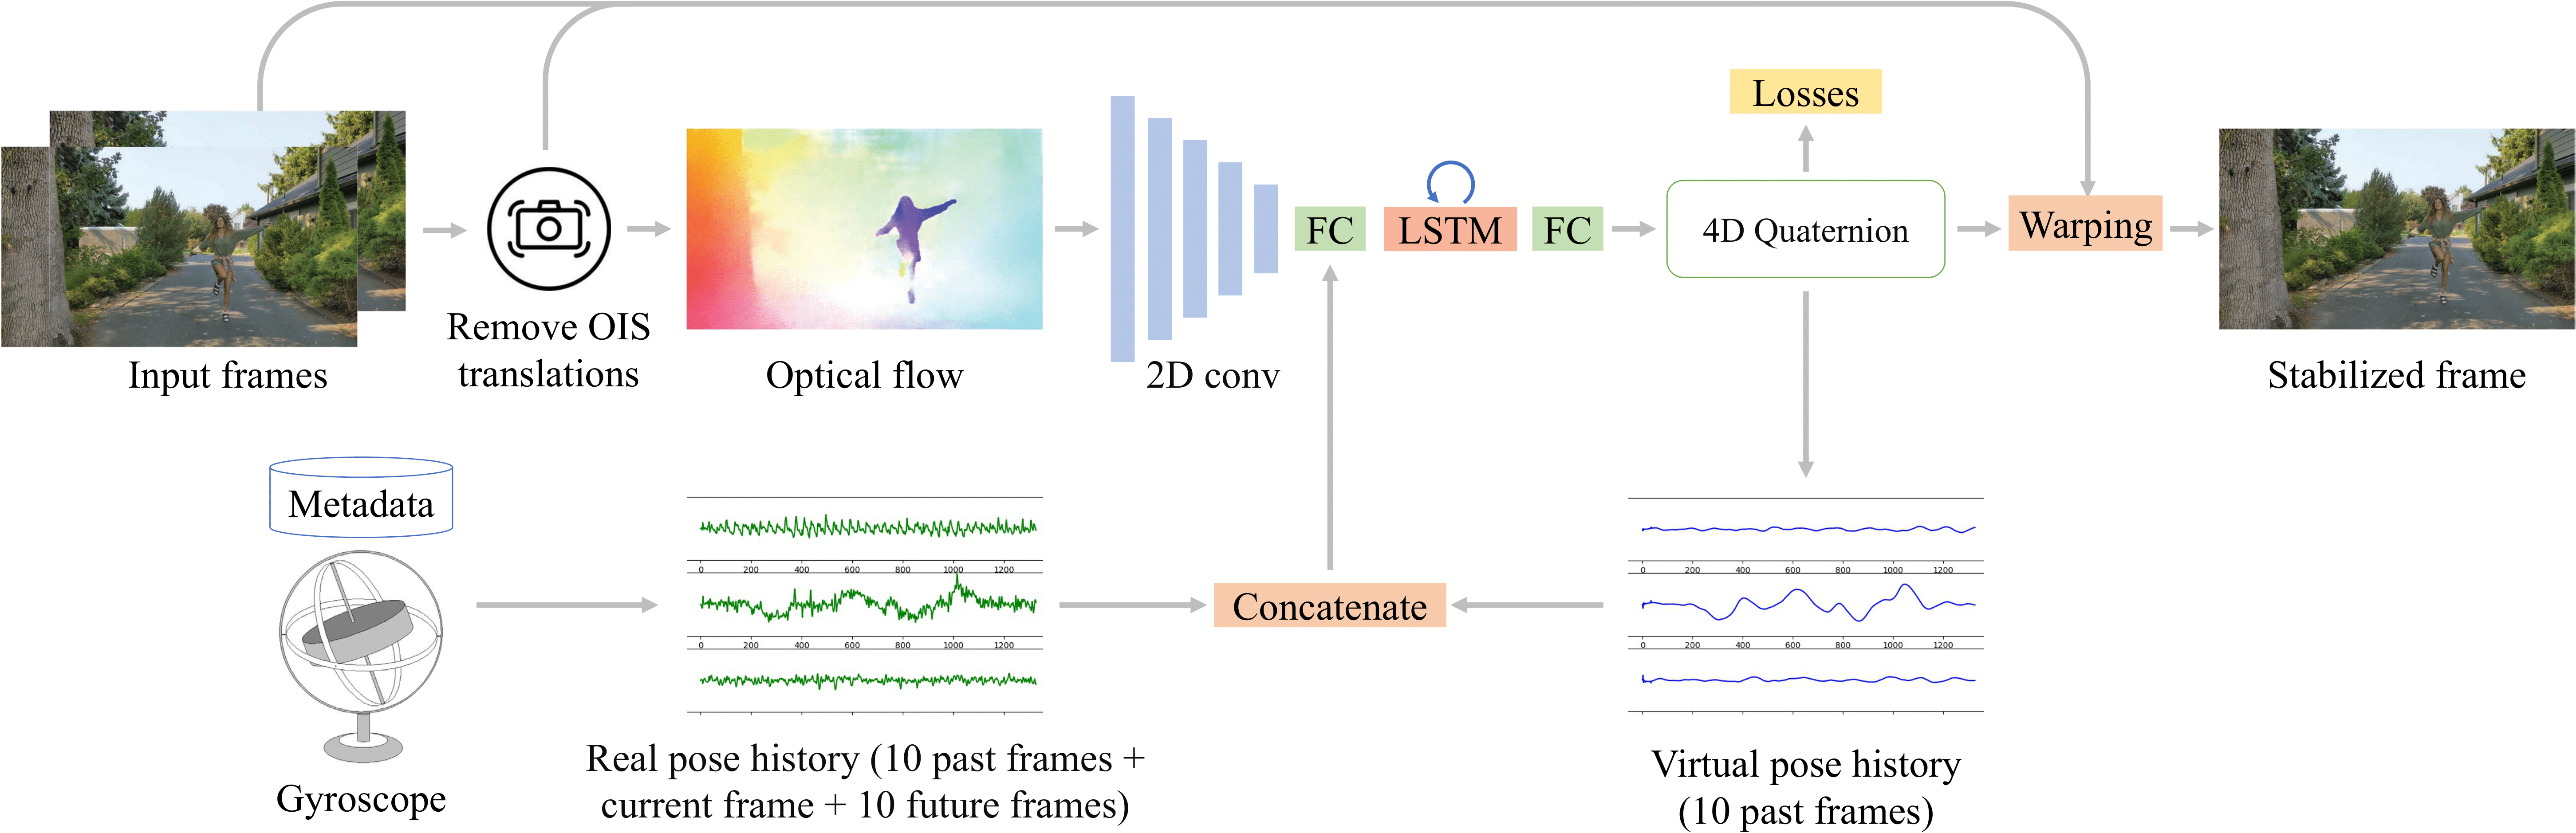
\includegraphics[scale=0.066]{images/fig_chapter3/deep_stab.png}
    \caption{Deep online fused video stabilization overview \citep{deep_opti_stab}}
    \label{fig:deep_stab}
\end{figure}

\section{Inertial Pose Estimation}
\label{sec:sota_pose_est}
Classical algorithms fail to accurately estimate the pose using MEMS IMU over a long period of time. With the advancement of artificial neural networks (ANNs) and their architectures new data driven techniques have been developed for this purpose. These data-driven techniques have outperformed their classical predecessors and are becoming a standard for this purpose. The drawback is that they are computationally very expensive and have very high edge hardware requirements. 

\subsection{RIDI: Robust IMU Double Integration}
RIDI was the first data-driven neural network approach which tackles the challenges of double integrating accelerometer readings. The algorithm regresses a velocity vector from the history of linear accelerations and angular velocities (IMU windows - discussed in section \ref{sec:data_structure}), then corrects low-frequency bias in the linear accelerations, which are integrated twice to estimate position \citep{yan2018ridi}. The analysis of results manifested that this algorithm outperformed the heuristic-based methods and even came closer to visual inertial navigation \citep{yan2018ridi}. The issue with this is it can only regress position and orientation estimation needs to be achieved using classical algorithms.

\subsection{RoNIN: Robust Neural Inertial Navigation in the Wild}
Developed by the same team as RIDI, RoNIN uses more advanced neural network architectures like ResNet, LSTM and TCN as its backbone to regress a velocity vecotor given a window of IMU samples \citep{herath2020ronin}. Input to the network in this case are the angular rates (Gyroscope readings), accelerations (accelerometer readings) and device orientations as shown in figure \ref{fig:ronin} and the output is motion trajectory (poses). Using these architectures and increasing the quality and size of data RoNIN outperforms RIDI and sets a new benchmark for inertial navigation \citep{herath2020ronin}. Our methodology is influenced by this technique and is discussed in chapter \ref{chapter_four} of this report.

\begin{figure}[H]
    \centering
    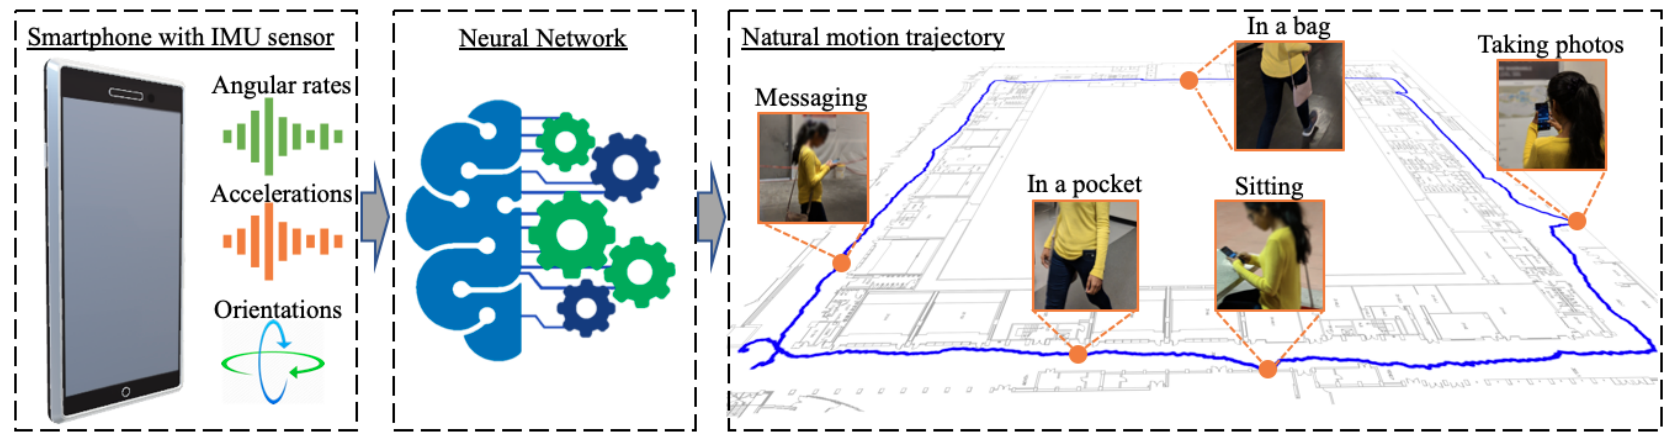
\includegraphics[scale=0.21]{images/fig_chapter3/ronin.png}
    \caption{RoNIN process layout \citep{herath2020ronin}}
    \label{fig:ronin}
\end{figure}

\subsection{TLIO: Tightly Learned Inertial Odometry}
This combines both classical and learn-based approaches by using an Extended Kalman Filter (EKF) and a deep neural network (DNN). The EKF is responsible for the prediction step while the outputs (displacement and uncertainty) from the neural network are used as a measurement update. The filter estimates rotation, velocity, position and IMU biases at IMU rate \citep{liu2020tlio} as shown in figure \ref{fig:tlio}. This approach is promising, but we were not able to reproduce the good results on our datasets, probably due to the difficult hyper-parameter settings that an EKF needs to perform well.

\begin{figure}[H]
    \centering
    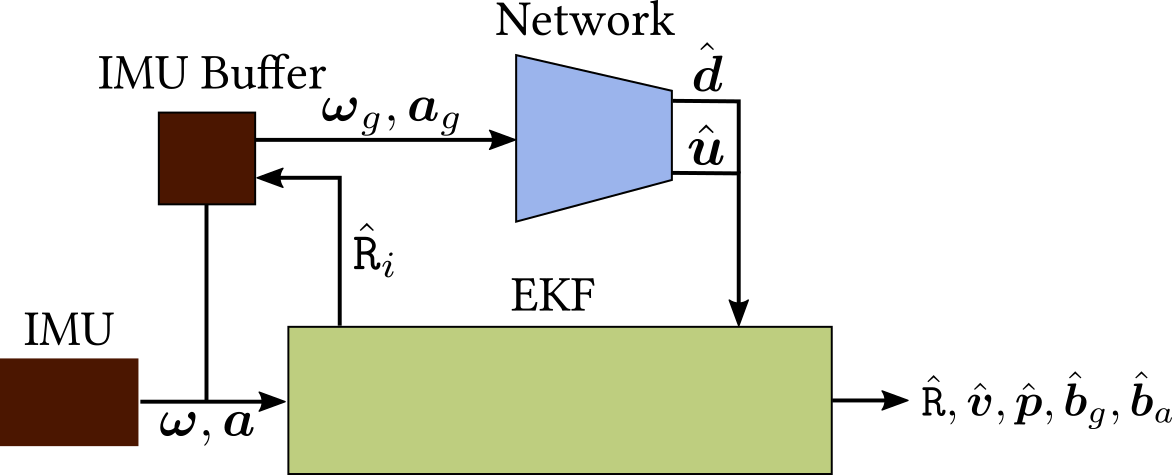
\includegraphics[scale=0.6]{images/fig_chapter3/tlio.png}
    \caption{TLIO architecture \citep{liu2020tlio}}
    \label{fig:tlio}
\end{figure}

\subsection{CTIN: Robust Contextual Transformer Network for Inertial Navigation}
This algorithm takes advantage of the recent advances in deep learning by using Multi-Headed-Attention (MHA) mechanism introduced in \citep{vaswani2017attention}. It uses a ResNet based encoder enhanced by local and global MHA to capture spatial contextual information from IMU measurements \citep{rao2022ctin} as shown in figure \ref{fig:ctin}. CTIN is claimed to be robust and to outperform state-of-the-art models but cannot be evaluated as it is not available publicly.

\begin{figure}[H]
    \centering
    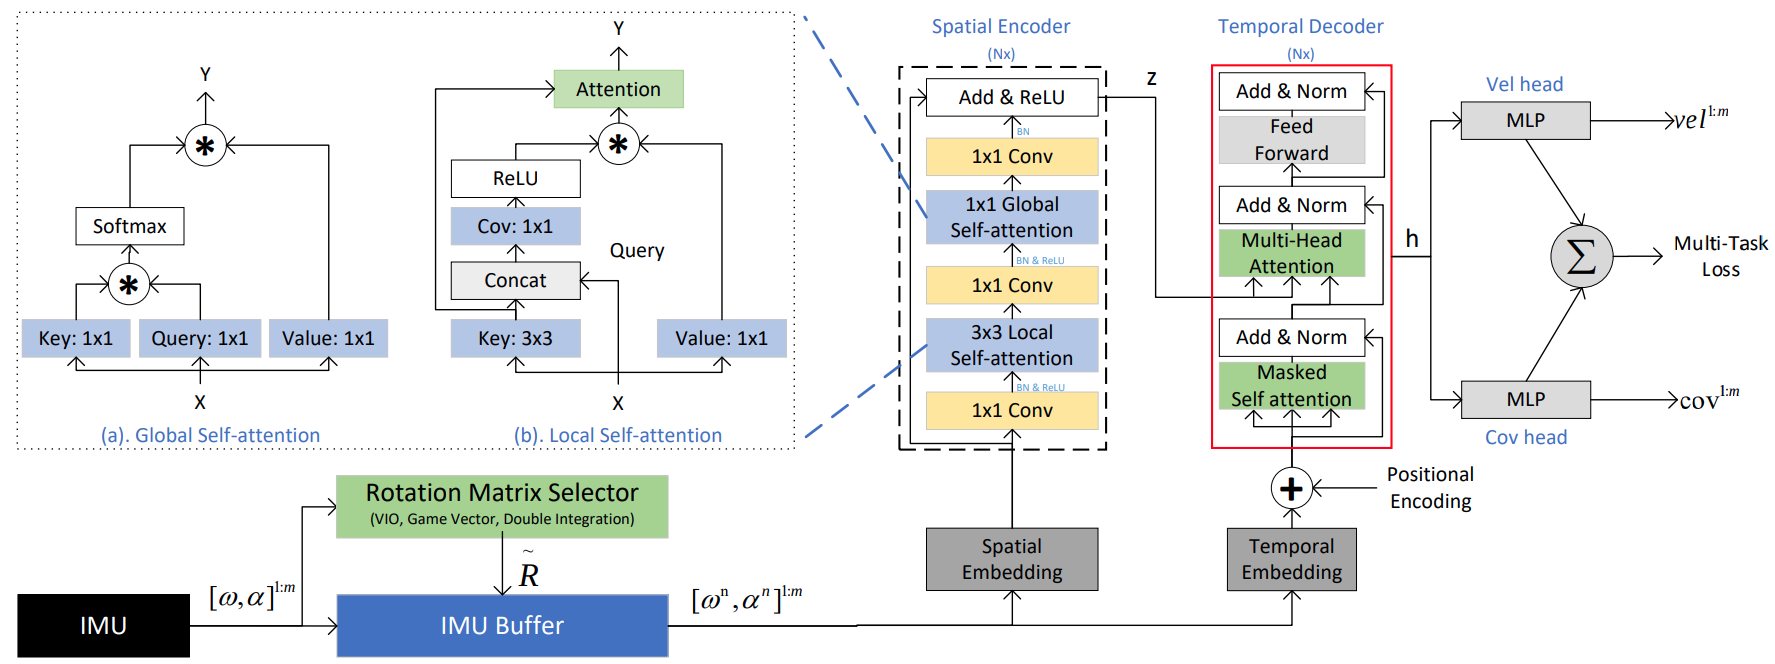
\includegraphics[scale=0.2]{images/fig_chapter3/ctin.png}
    \caption{CTIN Architecture \citep{rao2022ctin}}
    \label{fig:ctin}
\end{figure}



